\documentclass{rbfin}

%%%%%%%%%%%%%%%%%%%%%%%%%%%%%%%%%%%%
% INCIO DEL DOCUMENTO
%%%%%%%%%%%%%%%%%%%%%%%%%%%%%%%%%%%%
\begin{document}

\selectlanguage{brazil}
\frenchspacing

%%%%%%%%%%%%%%%%%%%%%%%%%%%%%%%%%%%%
% PORTADA
%%%%%%%%%%%%%%%%%%%%%%%%%%%%%%%%%%%%

% TÍTULO Y SUBTÍTULO DEL INFORME

\title{La descarbonización de la economía de Mendoza}
\otitle{Acciones en la economía del vino} 

% AUTORES
\author{
\bf{Buccolini Álvaro }%
 \email{alvarobuccolini@gmail.com}
\and
\bf{Isgro Ignacio }%
 \email{ignacioisgro12@gmail.com}
\and
\bf{Martínez y Arenas Lon }%
 \email{lonmartinez111@gmail.com}
  \and
\bf{Mellado Mauricio }%
 \email{maurimellado4@gmail.com}
 \and
\bf{Neme Omar }%
 \email{omarnemechacras@gmail.com}
}
% JOURNAL INFO
\maketitle
\pagina{1}

% ABSTRACT Y KEYWORDS
\begin{abstract}
\textbf{Abstract.}\ 
Este trabajo analiza la posibilidad de obtener financiamiento de la vid para el cumplimiento de los ODS 2030. Se considera que esta es una oportunidad importante de conseguir autoempleo para los egresados de ingeniería indus-trial como trabajadores free-lance de clase mundial, utilizando los fondos de la cooperación de la agencia alemana TGZ.

\textbf{Keywords.}
ODS 2030;
TGZ;
descarbonización.\\

\end{abstract}


%%%%%%%%%%%%%%%%%%%%%%%%%%%%%%%%%%%%
%SECCIÓN PRINCIPAL
%%%%%%%%%%%%%%%%%%%%%%%%%%%%%%%%%%%%
\section{Situación problema de Mendoza}\label{sec-intro}
 
 \lipsum[1-7]

\subsection{La vid}

\lipsum[1-2]

\begin{figure}
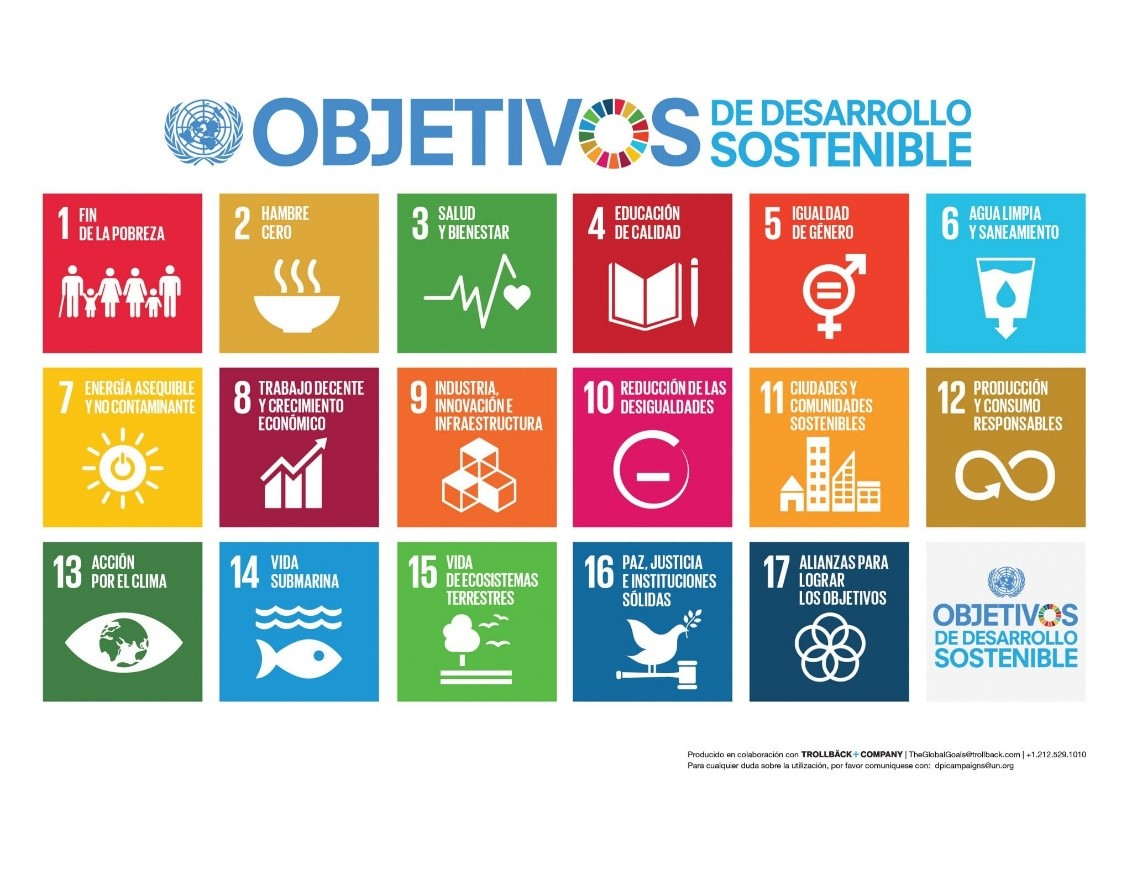
\includegraphics[width=\linewidth]{CEPAL.jpg}
 \caption{Los Objetivos de desarrollo según la CEPAL.}
  \label{fig:boat1}
\end{figure}

\lipsum[1-30]

\end{document}
%%%%%%%%%%%%%%%%%%%%%%%%%%%%%%%%%%%%
% FIN DEL DOCUMENTO
%%%%%%%%%%%%%%%%%%%%%%%%%%%%%%%%%%%%